\chapter{Implementierung}
\section{Konzeption und Methodik}


Das Konzept dieser Arbeit ist auf 3 Säulen aufgebaut. Erstens, das Sammeln, Speichern und Analyse der Daten und die Analyse der Daten, zweitens, das Entwickeln eines Deep Learning Modells, welches durch die gesammelten und angepassten Daten entsteht und drittens, das Implementieren und Einbetten des Modells in eine Benutzeroberfläsche, also in die Clientseite, siehe Abbildung~\ref{Kap5:Konzeption}.

\begin{figure}[H]
    \centering
    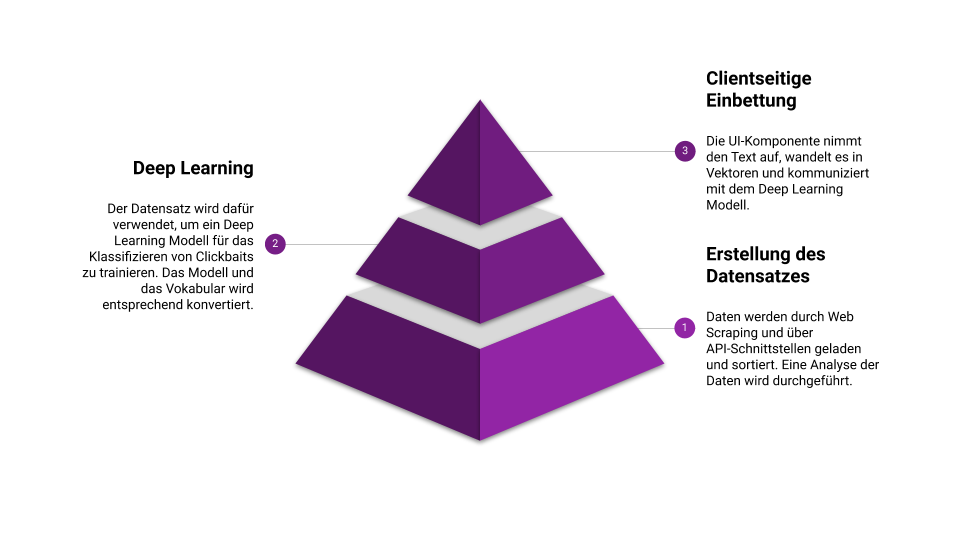
\includegraphics[width=15cm]{kapitel5/main_p.png}
    \caption[Darstellung der Konzeption]{Darstellung der Konzeption}
    \label{Kap5:Konzeption}
\end{figure}


Deep Learning Modelle benötigen eine große Menge an Beispielen um zu lernen. Es reicht außerdem nicht aus, nur eine große Menge an Daten zu beschaffen, sondern auch gute Daten auszuwählen. In der Studie von \cite*{Chakrabortya} haben die Autoren Daten aus dem Web geladen. Für die erste Kategorie, der Nicht-Clickbaits, wurde die Wikipedia-News-API verwendet. Um genug Beispiele für Clickbaits zu finden, sollten solche Medien herausgefunden werden. Um die Daten labeln zu können ist neben dem Titel eines Datenelementes auch die extraktion der Nachricht zu erfassen.

Die Wikipedia-News-API bietet einen Kostenlosen Endpunkt an, welches verschiedene Nachrichtenportale wie z.B. Politik, Wirtschaft, Kultur, Sport und Wissenschaft anbietet. Um Clickbaits zu finden verläuft die Datenaquise wesentlich schwieriger. Der Datensatz von \cite*{Chakrabortya} beinhalter jeweils 7500 Nachrichten je Kategorie. Es ist zu berücksichtigen, dass diese nicht mit Deep Learning Modellen arbeiten, sondern mit klassischen Machine Learning Algorithmen, die weniger Daten benötigen. Es müssen also mehr Daten her, also die Suche sollte neben den klassischen Clickbait-Seiten auch woanders erfolgen. Um die Datenextraktion zu automatisieren bietet sich die Software \enquote{Scrapy} an. Scrapy ist ein Open-Source Tool, welches das extrahieren von großen Mengen an Daten erleichtert. Es ist in Python geschrieben und kann durch seine Middleware Funktion auch die Daten direkt in eine SQL-Datenbank speichern.

Der mittlere Kern der Pyramide in Abbildung~\ref{Kap5:Konzeption} ist das Deep Learning Modell, welches als Inferenzmaschine betrachtet werden kann. Es wird durch Eingabe von gelabelten Daten trainiert und in ein entsprechendes Format gebracht. Es gibt mehrere Anbieter für das Deep Learning. Die meisten von Ihnen sind Open Source. Die bekanntesten Bibliotheken für das Deep Learning sind TensorFlow (welches von Google unterstützt wird) und PyTorch (welches von Facebook unterstützt wird). Seit März 2018 bietet TensorFlow die Möglichkeit, Modelle in der Programmiersprache JavaScript zu trainieren und zu benutzen. Ein klassischer Vorgang um Deep Learning Modelle dem Endbenutzer durch Webprogrammierung anzubieten war es immer, dass zunächst ein Modell trainiert wurde und dann auf einem Server geladen wurde. Der Server hatte dann einen Endpunkt, z.B. eine POST-Anfrage, welches eine Anfrage vom Clienten empfang. Diese Anfrage wurde dann im Server durch das Modell beantwortet und der Server sendete dem Clienten das Ergebnis. Durch TensorFlow.js ist es möglich erstens ein Modell komplett auf der Programmiersprache JavaScript zu entwickeln und zweitens es die Inferenzbildung durch einen Server in der Mitte nicht mehr nötig. Das Modell kann zusammen mit dem Framework in den Browser geladen werden und die bearbeitung erfolgt dort. In dieser Arbeit wurde das Modell nicht mit TensorFlow.js trainiert, da es auch möglich ist, Modelle in der konventionellen Weise mit der Keras API zu trainieren und dann in ein Webfreundliches Format umzuwandeln. Nach der Konversion können die Gewichte welches das Modell gerechnet hat und eine JSON-Datei, welches das Modell beschreibt hochgeladen und benutzt werden. Der Client muss nur noch diese Dateien in den Browser laden und kann dann selbst die Anfrage beantworten. Das trainieren auf konventionellen Wegen bietet außerdem den Vorteil, dass die Umgebung auf JavaScript nicht mit der Umgebung in Python konkurrieren kann. Die meisten Tools und Frameworks werden für Python geschrieben. Ein weiterer Grund ist, dass die bearbeitung auf dem heimischen Computer sehr langsam ist. Mit Google Colab können Deep Learning Modelle mit viel Rechnerkapazität trainiert werden.

Die Spitze der Pyramide macht die Benutzeroberfläsche aus. Diese wird komplett in JavaScript geschrieben. JavaScript ist die meistbenutze Programmiersprache und wird heute neben Webentwicklung auch auf dem Server verwendet. Mit TensorFlow.js ist es nun auch möglich, mit Tensors umzugehen. Die Schwierigkeit hier ist es, den Text, den der Benutzer eingibt, in Token und dann diese Token in Vektoren umzuwandeln, wenn das Modell keinen sogenannten \enquote{Input-Layer} hat welches einfache String einnehmen kann und diese umwandeln kann, dieses macht das Modell aber viel größer, da es eine größere Anzahl an Parametern hat und nicht Ziel dieser Arbeit. Eine andere Möglichkeit ist es, das gesamte Vokabular in einer JSON-Datei zu speichern und es der Benutzeroberfläsche zugänglich zu machen. Jedes auftauchende Wort im Vokabular bekommt einen Index, welches dann als \enquote{Übersetzer} dient und zur Umwandlung der Strings in Vektoren verwendet werden.




\section{Erstellung des Datensatzes}
\subsection{Erste Rohdatenbeschaffung durch Web Scraping}

Um einen Forschungsbeitrag zu leisten, hat diese Arbeit das Ziel ein Clickbait Corpus auf deutscher Sprache zu erstellen. Für die Erstellung eines solchen Korpus sind zunächst bestimmte Seiten einzugrenzen, die Clickbait Nachrichten anbieten. Die bekannteste Seite ist \enquote{buzzfeed} und \enquote{tasty}. Außerdem wurden auch Webseiten wie \enquote{web.de} oder \enquote{tv-movie}\footnote{Beinhaltet außerdem Schlagzeilen aus den Bereichen \enquote{tasty} und \enquote{quiz}} nach Clickbaits gescannt. Das Screening wurde am November 2020 durchgeführt. Um jedoch zu gewährleisten, dass die Nachrichten zeitlich weit außereinder liegen und somit eine größere Diversität haben, wurden Webseiten ausgewählt die Ihre Nachrichten in gewisser Weise Archivieren. Die gesammelten Daten reichen teilweise über ein Jahr zurück. Wie im Listing~\ref{Scrapy} unter in Zeile 12 zu sehen ist, besitzt die Seite im Beispiel eine Pagination-Funktion. Diese kann dafür verwendet werden, um auch ältere Nachrichten zu erfassen.

\begin{table}[h]
    \caption{Vergleich der Rohdaten nach dem Scrapingvorgang}
    \label{Datensatz_Herkunft}
    \renewcommand{\arraystretch}{1.2}
    \centering
    \sffamily
    \begin{footnotesize}
        \begin{tabular}{l l l}
            \toprule
            \textbf{Quelle}   & \textbf{Methodik} & Elemente \\
            \midrule
            de.wikinews.org   & API-Zugang        & 10.612   \\
            web.de            & Web Scraping      & 14.163   \\
            tvmovie.de        & Web Scraping      & 9.428    \\
            buzzfeed.de       & Web Scraping      & 798      \\
            promipool.de      & Web Scraping      & 26.779   \\
            heftig.de         & Web Scraping      & 605      \\
            frauenseite.net   & Web Scraping      & 148      \\
            bravo.de          & Web Scraping      & 7.476    \\
            \midrule
            Summe Clickbaits  &                   & 59.407   \\
            Summe Nachrichten &                   & 10.612   \\
            Summe insgesamt   &                   & 70.019   \\
            \bottomrule
        \end{tabular}
    \end{footnotesize}
    \rmfamily
\end{table}



Das Verfahren wurde automatisch mittels eines programmierten Scrapers je Seite durchgeführt. Ein Scraper ist ein Programm, welches Informationen aus einer Webseite automatisch extrahieren kann. Dieses gelingt, indem es nach HTML- oder CSS-Attributen oder sogar AJAX-Requests durchsucht oder diese imitiert. Im Listing~\ref{Scrapy} wird ein Web-Scraper vorgestellt. Scrapy führt in einer Schleife HTTP-Requests durch welche jeweils eine Antwort bekommen. Es können auch AJAX-Anfragen gesendet werden (z.B. ein POST-Request). Wenn die Anfrage Erfolgreich ist, kann die daraus resultierende Antwort auf bestimmte Eigenschaften und Attribute durchsucht werden (im Beispiel werden CSS-Attribute durchsucht). Diese Attribute beinhalten meisten die gewünschte Information, welches dann wie in der \texttt{parse\_url} und \texttt{parse\_page} Methode gezogen und in eine Datenbank gespeichert wird.



\begin{lstlisting}[language=Python,caption=Beispiel eines Scrapers]
import scrapy
from scrapy.http.request import Request
from datetime import datetime
from klickscraper.items import WebdeItem


class WebdeSpider(scrapy.Spider):
    name = "webde"
    scraped_at = datetime.now()

    def start_requests(self):
        for i in range(287):
            url = f"https://web.de/magazine/unterhaltung/stars/p{i}"
            yield Request(
                dont_filter=True,
                callback=self.parse_url,
                url=url)

    def parse_url(self, response):
        follow_ulrs = response.css(
            ".teaser-article__full").css("a::attr(href)").getall()
        for f in follow_ulrs:
            yield Request(
                url=f,
                dont_filter=True,
                callback=self.parse_page)

    def parse_page(self, response):
        if len(response.css("p::text").getall()) > 10:
            text = " ".join(response.css("p::text").getall())
        else:
            text = None
        yield WebdeItem(title=response.css('title::text').get(),
                        text=text,
                        scraped_at=self.scraped_at)
\end{lstlisting}\label{Scrapy}


\subsection{Explorative Datenanalyse der Rohdaten}
Um aus den Rohdaten Schlüsse über die sprachlichen Eigenschaften zu ziehen wird im folgenden Abschnitt eine explorative Datenanalyse durchgeführt. Um dies möglichst zu vereinfachen, wird der Rohdatensatz welches in einer SQL-Datenbank gespeichert wurde in ein Pandas\footnote{Pandas ist ein schnelles, flexibles und benutzerfreundliches Open-Source-Tool zur Analyse und Bearbeitung von Daten in Python.} Dataframe umgewandelt.
Aus der Abbildung~ist zu sehen, dass die Titel aus Wikinews länger sind. Neben der Länge der Schlagzeilen ist auch die Analyse der Wortauswahl wichtig. Aus der Literaturstudie können bestimmte Merkmale von Clickbaits festgestellt werden. Clickbaits enthalten meistens eine Frage oder Zahlen. Außerdem ist bei Clickbaits auch eine gewisse Wortauswahl festzustellen. Die Zuordnung der Wörter je Clickbait-Schlagzeile zu den Wortarten (Part-of-speech-Tagging oder POS-Tagging) wurde mittels der Python NLP-Bibliothek Spacy durchgeführt. Bei der Auswahl der Tags nachdem gesucht werden sollte, wurden die Erkenntnisse aus Kapitel 4 Berücksichtigt. Die Ergebnisse diese Analyse sind aus der Tabelle~\ref{pos} zu entnehmen.

\begin{table}[h]
    \caption{Vergleich der Ergebnisse des Part-of-speech-Taggings}
    \label{pos}
    \renewcommand{\arraystretch}{1.2}
    \centering
    \sffamily
    \begin{footnotesize}
        \begin{tabular}{l l l}
            \toprule
            \textbf{TAG}                  & \textbf{Auffälliges Wort (Häufigkeit)} \\
            \midrule
            ADJA  (attributives Adjektiv) & neu (1759), neue (1474)                \\
            ADJD   (adverbiales Adjektiv) & krass (171), wirklich  (349)           \\
            ADV   (Adverb)                & so (5142), endlich (357)               \\
            PDAT (Demonstrativpronomen)   & dies (3566)                            \\
            PROAV   (Pronominaladverb)    & darum (588), deshalb (251)             \\
            PWAT (Interrogativpronomen)   & welch (154)                            \\
            PWAV  (Relativpronomen)       & wie (488) warum (184)                  \\
            \bottomrule
        \end{tabular}
    \end{footnotesize}
    \rmfamily
\end{table}

% Eine eigene Analyse durch das Part-of-Speech_tagging mittels Scrapy ergibt einige Auffälligkeiten bezüglich der Clickbaits. Wörter wie \enquote{diese} (attribuierendes Demonstratives Pronomen), \enquote{warum} (adverbiales Interrogativ- oder Relativpronomen) oder \enquote{welche} (attribuierendes Interrogativpronomen) sind einige Auffällige Tags aus den Schlagzeilen der Clickbaits.



% \begin{lstlisting}[language=Python,caption=Funktion zur Umwandung der Datenbank in en Pandas Dataframe]
% def connect_to_db(tablename, db_path):
%     return pd.read_sql_query(
%         f"SELECT * FROM {tablename}", sqlite3.connect(db_path))
% \end{lstlisting}\label{Pandasdb}


\begin{figure}[H]
    \centering
    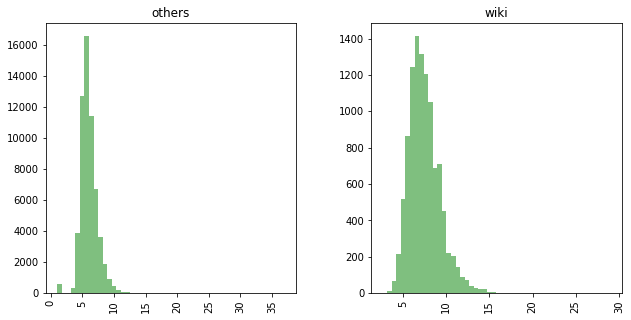
\includegraphics[width=14cm]{kapitel5/hist2.png}
    \caption[Vergleich der Wortlängen der Rohdaten]{Vergleich der Wortlängen, das Histogramm rechts (Wikinews) ist breiter als das Histogramm links (Clickbaits)}
    \label{Kap5:Hist2}
\end{figure}

% \begin{figure}[H]
%     \centering
%     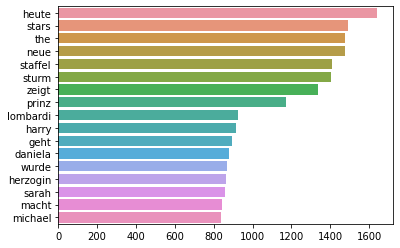
\includegraphics[width=10cm]{kapitel5/freq_word1.png}
%     \caption[Häufigsten Wörter aus den Rohdaten der Clickbaits Titel]{Die Darstellung zeigt das Aufkommen der Häufigsten Wörter aus den Titeln der Clickbaits}
%     \label{Kap5:freq1}
% \end{figure}

% \begin{figure}[H]
%     \centering
%     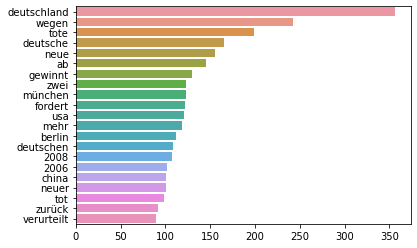
\includegraphics[width=10cm]{kapitel5/freq_word2.png}
%     \caption[Häufigsten Wörter aus den Rohdaten der Wikinews Titel]{Die Darstellung zeigt das Aufkommen der Häufigsten Wörter aus den Titeln der Wikinews Nachrichten}
%     \label{Kap5:freq2}
% \end{figure}


\subsection{Labeln der Daten}
Aus der Tabelle~\ref{Datensatz_Herkunft} ist zu entnehmen, dass ca. 60.000 potenzielle Clickbaits vorhanden sind. Um dieses nicht per Hand labeln zu müssen besteht der Ansatz darin, bestimmte Muster zu erkennen und diese Muster auszunutzen, um die Anzahl der Kandidaten auf ein entsprechendes niedriges Niveau zu bringen. Die Literaturstudie und die explorative Datenanalyse bringen gemeinsam folgende Schlüsse:

\begin{enumerate}
    \item Clickbaits sind meisten Fragen wie \enquote{Welcher Schuh passt dir am meisten?}
    \item Clickbaits enthalten meistens Zahlen in Form eines Listings \enquote{Das sind die 10 schnellsten Autos}
    \item Clickbaits haben eine niedrigere Wortlänge als normale Nachrichten
    \item Clickbaits beinhalten einige für sie markanten Wörter wie \enquote{diese} oder \enquote{so}
\end{enumerate}

Diese Erkenntnisse können programmatisch umgewandelt werden und somit der Rohdatensatz um ein vielfaches reduziert werden.


\begin{lstlisting}[language=Python,caption=Funktion welches ein Dataframe je nach Argumenten labelt]
def contains_word(word, row):
    for r in row:
        if r in word:
            return 1


def label_data_with_arg(df, col_name, arg_):
    return df[col_name].apply(
        lambda x: contains_word(arg_, re.findall(r"[\w']+|[.,!?;]", x.lower())))
\end{lstlisting}\label{Label1}

\begin{lstlisting}[language=Python,caption=Funktionen für durchschnittliche Wortlänge und Interpunktion]
import re
import string

def remove_punc(text):
    text = re.sub('\[.*?\]', '', text)
    text = re.sub('https?://\S+|www\.\S+', '', text)
    text = re.sub('<.*?>+', '', text)
    text = re.sub('[%s]' % re.escape(string.punctuation), '', text)
    text = re.sub('\n', '', text)
    text = re.sub('\w*\d\w*', '', text)
    return text

def get_avg_length(string):
    words = remove_punc(string).split()
    try:
        count = int(sum(len(word) for word in words) / len(words))
    except ZeroDivisionError:
        count = 1
    return count
\end{lstlisting}\label{Label2}

\begin{lstlisting}[language=Python,caption=Tagger Funktion]
import spacy
nlp = spacy.load('de')

def contains_pos(sentence):
    list_ = ["PDAT", "ADJD", "ADJA", "PIS", "PWAV", 
            "PTKA", "VAFIN", "PROAV", "ADV"]
    doc = nlp(sentence)
    for token in doc:
        if str(token.tag_) in list_:
            return "1"

def label_data_with_pos(df, col_name):
    return df[col_name].apply(
        lambda x: contains_pos(x.lower()))
\end{lstlisting}\label{Label3}


\subsection{Analyse der Daten}
Die Summe der Wikinews Nachrichten beträgt ca. 10.000. Mit der Zugabe weiterer 10.000 Clickbaits, die durch das labeln entstehen, ergibt sich ein Datensatz mit 20.000 Beispielen. Die Tabelle~\ref{data} verschafft einen Übrerblick über alle Daten. Interessant ist bei den Clickbaits, dass ca. 33\% aller Clickbaits ein Fragezeichen oder eine Zahl beinhalten und ca. die hälfte aller Daten im Datensatz ein bestimmtes Tag wie \enquote{diese} oder \enquote{so} enthalten. Bei den Wikinews Nachrichten liegen diese Anteile deutlich unten. Alle drei genannten Eigenschaften liegen unter 1\%. Die durchscnittliche Wortlänge beträgt bei den Clickbaits bei 5, während bei den Wikipedia Nachrichten dieses bei 7 liegt.

\begin{table}[h]
    \caption{Beschreibung des gelabelten Datensatzes}
    \label{data}
    \renewcommand{\arraystretch}{1.2}
    \centering
    \sffamily
    \begin{footnotesize}
        \begin{tabular}{l l l l l l}
            \toprule
                           & \textbf{has\_question} & \textbf{has\_keyword} & \textbf{has\_number} & \textbf{avg\_word\_length} & \textbf{label} \\
            \textbf{count} & 20000                  & 20000                 & 20000                & 20000                      & 20000          \\
            \textbf{mean}  & 0.1782                 & 0.3190                & 0.0854               & 6.1307                     & 0.5000         \\
            \textbf{std}   & 0.3826                 & 0.4661                & 0.2795               & 1.7874                     & 0.5000         \\
            \textbf{min}   & 0                      & 0                     & 0                    & 1.0000                     & 0              \\
            \textbf{max}   & 1                      & 1                     & 1                    & 27.0000                    & 1              \\

            \bottomrule
        \end{tabular}
    \end{footnotesize}
    \rmfamily
\end{table}

Bei der Betrachtung der Wörter mit der Word-Cloud Analyse können bestimmte Themen, die die Titel zürückgeben betrachtet werden.  Auffällig sind neben Promis auch die Wörter \enquote{darum}, \enquote{quiz} \enquote{sieht} und \enquote{macht}. Bei den Wikipedia Nachrichten geht es mehr um Deutschland und der Welt.


\begin{figure}[H]
    \centering
    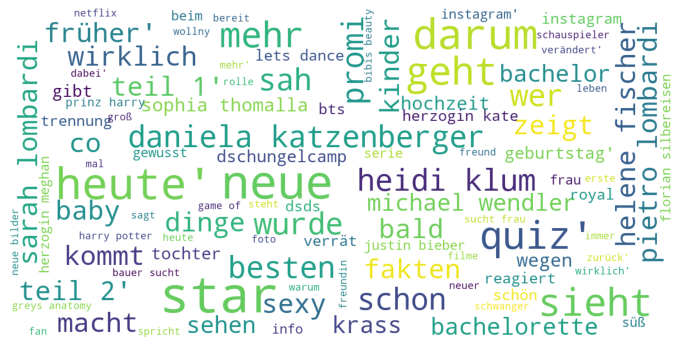
\includegraphics[width=12cm]{kapitel5/wo_click.png}
    \caption[Word Cloud Analyse für die Clickbaits Schlagzeilen]{Die Darstellung zeigt das Aufkommen der Häufigsten Wörter aus den Titeln der Wikinews Nachrichten}
    \label{Kap5:clwc}
\end{figure}

\begin{figure}[H]
    \centering
    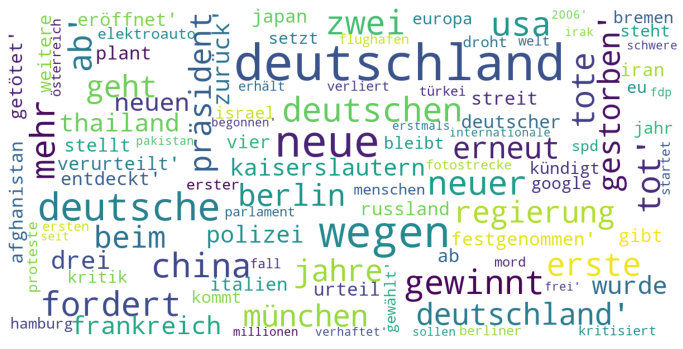
\includegraphics[width=12cm]{kapitel5/news.png}
    \caption[Word Cloud Analyse für die Wikinews Schlagzeilen]{Die Darstellung zeigt das Aufkommen der Häufigsten Wörter aus den Titeln der Wikinews Nachrichten}
    \label{Kap5:clwc}
\end{figure}


\section{Das Deep Learning Modell}
\subsection{Einleitung}
\subsection{Soft- und Hardware}
\subsection{Preporcessing}
\subsection{Tokenisierung}
\subsection{Embedding Layer}
\subsection{Das CNN-Model}
\subsection{Training und Evaluation}
\subsection{Umwandlung und Export in ein Webformat}
%(mit Vocab.json)
\subsection{Schluss}
